% File tacl2018v2.tex
% Sep 20, 2018

% The English content of this file was modified from various *ACL instructions
% by Lillian Lee and Kristina Toutanova
%
% LaTeXery is mostly all adapted from acl2018.sty.

\documentclass[11pt,a4paper]{article}
\usepackage{times,latexsym}
\usepackage{url}
\usepackage[T1]{fontenc}
\usepackage{graphicx}

%% Package options:
%% Short version: "hyperref" and "submission" are the defaults.
%% More verbose version:
%% Most compact command to produce a submission version with hyperref enabled
%%    \usepackage[]{tacl2018v2}
%% Most compact command to produce a "camera-ready" version
%%    \usepackage[acceptedWithA]{tacl2018v2}
%% Most compact command to produce a double-spaced copy-editor's version
%%    \usepackage[acceptedWithA,copyedit]{tacl2018v2}
%
%% If you need to disable hyperref in any of the above settings (see Section
%% "LaTeX files") in the TACL instructions), add ",nohyperref" in the square
%% brackets. (The comma is a delimiter in case there are multiple options specified.)

%\usepackage[]{tacl2018v2}
\usepackage[acceptedWithA]{tacl2018v2}

%%%% Material in this block is specific to generating TACL instructions
\usepackage{xspace,mfirstuc,tabulary}
\newcommand{\dateOfLastUpdate}{Sept. 20, 2018}
\newcommand{\styleFileVersion}{tacl2018v2}

\newcommand{\ex}[1]{{\sf #1}}

\newif\iftaclinstructions
\taclinstructionsfalse % AUTHORS: do NOT set this to true
\iftaclinstructions
\renewcommand{\confidential}{}
\renewcommand{\anonsubtext}{(No author info supplied here, for consistency with
TACL-submission anonymization requirements)}
\newcommand{\instr}
\fi

%
\iftaclpubformat % this "if" is set by the choice of options
\newcommand{\taclpaper}{final version\xspace}
\newcommand{\taclpapers}{final versions\xspace}
\newcommand{\Taclpaper}{Final version\xspace}
\newcommand{\Taclpapers}{Final versions\xspace}
\newcommand{\TaclPapers}{Final Versions\xspace}
\else
\newcommand{\taclpaper}{submission\xspace}
\newcommand{\taclpapers}{{\taclpaper}s\xspace}
\newcommand{\Taclpaper}{Submission\xspace}
\newcommand{\Taclpapers}{{\Taclpaper}s\xspace}
\newcommand{\TaclPapers}{Submissions\xspace}
\fi

%%%% End TACL-instructions-specific macro block
%%%%

% \title{Formatting Instructions for TACL \TaclPapers \\
% (Base files: \styleFileVersion-template.tex \& \styleFileVersion.sty, dated \dateOfLastUpdate)}
\title{Text classifications using IMapBook dataset}


% Author information does not appear in the pdf unless the "acceptedWithA" option is given
% See tacl2018v2.sty for other ways to format author information
\author{
 Domen Kos, Timotej Kovač \\
 University of Ljubljana \\
 Faculty of computer and information science \\
 Večna pot 113, SI-1000 Ljubljana \\
  {\sf dk6314@student.uni-lj.si, tk3713@student.uni-lj.si} \\
}

\date{}

\begin{document}
\maketitle
 \begin{abstract}
In this paper we discuss our various approaches when trying to classify messages from an IMapBook dataset.
We dive into some of the traditional nature language processing approaches like using Logistic Regression, Support Vector Machine and also adding our own rules along with some more recent ones like the use of reccurent neural networks or transformers.
 \end{abstract}


\section{Introduction}
For the course assignment at \textit{Natural language processing} class we decided to do text classification on IMapBook dataset.
The dataset contains short discussions between primary school students who are chatting about different book topics.
Each record is annotated with 16 attributes.
Original messages are posted in Slovene language, but they are also translated to English.
We also have the information about topic they are discussing, if their message was an answer to some previous asked question and if their discussion is relevant to the topic, since there are no constraints so they can write anything they want.
If the discussion is moving away from the proposed topic, the teacher can intervene and guides it back by asking some questions relevant to the book.
Dataset contains approximately 3500 messages about 3 different short stories.
Our goal is to develop the models which could detect the topic of the current debate so the teacher can intervene.
The idea is to develop different models and combine their outputs.
We would analyse conversation on different levels.
First would be to analyse separate messages and define their relevance to the topic.
We would also define type of message which can either be answer or question and also the category.
By combining results of separate messages we could determine when the conversation is starting to move away from the topic.

\section{Related work}
Text classification is a popular topic of natural language processing (NLP) field, thus there are many researchers working on the field. In this section we present most relevant work and techniques they used.

Most of the research work and the state-of-the-art results were achieved using English language, but some of the techniques and approaches can be adapted to Slovene language.
The authors of paper~\cite{articleSpanish} had similar problem, where they analysed Spanish tweets which are also relative short texts.
They discuss different approaches for preprocessing data to extract the most relevant features which are later used for classification.
Few standard approaches are discussed like how to define a basic term which are used by classification algorithms.
Such as uni-grams (1-grams), bi-grams (2-grams), tri-grams (3-grams), n-grams.
They found out that having n larger than 3 does not improve results.
They also tried combining different types of n-grams (like uni-grams and bi-grams) to achieve better results.
That also means that attribute list was larger so they removed some entries by setting a threshold value.
With threshold they removed n-grams that did not appear frequently enough or they appeared to many times, since they were considered as noise.
They also discuss how important are stemming and lemmatization comparing English and Spanish language which is also interesting for Slovene language which is also morphological richer then English.

In second paper~\cite{article2} authors presented the recurrent convolutional neural network for text classification.
The network was able to capture contextual information of the sentence and extract features and learn some word representation.
As described the disadvantage of the recurrent network is that although the context of the word is captured, the model is biased where later words are more dominant then earlier.
To tackle this problem they applied additional convolutional and pooling layers.
They learned a word Representation and used it for some text classification.

Another similar approach is used in third paper~\cite{article3} where the authors used convolutional neural networks for text categorization where the word order was also taken into account.
The input to the network is not standard bag-of-word representation but they present their own word representations which are some higher dimensional vectors where 2D convolution is applied.
For baseline model they used a support vector machine (SVM) classifier with bag-of-word representation and showed that their approach gave them lower error rate than standard models.

There are also many already pre-trained word representations which can be used, also for Slovenian language.
The word embeddings induced from a large collection of Slovene texts composed of existing corpora of Slovene were prepared and published on CLARIN~\cite{embeddings}.
This could also be useful with our task since the embeddings were learned on bigger corpuses then are available to us.

\section{Initial ideas}

To determine if the teacher must intervene we need to answer the following questions:
\begin{itemize}
\item{are the messages book relevant,}
\item{what type is the message,}
\item{in what category does it belong.}
\end{itemize}

Based on this information we could then determine if the conversation is in need of an intervention or not.

Because there are three seperate requirements our first idea was to come up with three seperate classifiers.
We will start with standard text classification procedures like tokenizing, stemming, removal of stop words and then represented words as vectors in order to use them in our machine learning algorithms.
After that we will probably use some kind of machine-learning approach. 
Recurring convolutional neural networks or SVMs could be used to make use of the sequential information of words as well.

\subsection{Book relevance}
Here the answer we are trying to answer is whether the message is related to a story or not.
From the data itself came to some conclusions:

\begin{itemize}
\item{Category of the message is a good indication whether the message is book relevant. 
So if the message is classified as having a category discussion it is a good chance that the message is book relevant.
So the result of the message category classifier could be used here to determine if the book is relevant.}
\item{Conversations have some retention.
If the conversation starts leaning towards a discussion of a book most messages will be about the book, and if the conversation starts to move towards some other category most of the messages will follow.
So here the sequence and previous states could be deemed important.}
\end{itemize}

A good idea would be to include the original texts from the three books that our gathered messages are reffering to.
Another possible approach to clasify book relevance would be to use the result of the message category (see section Message category) in order to get better results.

\subsection{Type of the message}
Here we try to answer the type of the message. 
This can be a statement, a question or an answer.
Here too we drew some conclusions from the data available:

\begin{itemize}
\item{Answers tend to follow questions. So message order is important.}
\item{Answers are mostly regarded as book relevant and statements are not.}
\end{itemize}

Determening questions can be done by adding a feature that checks if the sentence contains a question mark or some sort of question word.
To determine answers from statements we will most likely have to take into account the order of sentences as well.

\subsection{Message category}

Each message can be one of the following:
\begin{itemize}
\item{\textbf{chatting}, which doesn't fall into any of the bellow categories;}
\item{\textbf{switching}, which mostly consists of asking for help;}
\item{\textbf{discussion}, which consists of some particular keywords ('lahko', 'bi) and descriptions of activities, objects;}
\item{\textbf{moderating}, where the teacher leads the converstation and which we could identify by maybe checking for gramatically correct sentences;}
\item{\textbf{identity}, where we could check the appearance of question marks or question words or}
\item{\textbf{other}, where there is mostly gibberish.}
\end{itemize}

Some manual features could be added which would be especially efficient for determining the categories \textbf{other} and \textbf{identity}.
Very long words or those that contain a single repeating character can quickly be classified as "other" as well as those that only contain emojis or other special characters.
Detecting question marks, question words and possibly personal names can largely contribute to classifing message as being of type identity.

\section{Experiments}
In this section we present the pre-processing steps we performed and all the experiments we performed.

\subsection{Text pre-processing}
We followed some standard text pre-processing steps.
First we tokenized each chat.
After that we used lemmatizer to get the basic forms of each token.
Both of the steps were first performed using the standard NLP tools which are available mostly for English language.
Since Slovene language is a bit different the tokenization and lemmatization were not always correct.
For that reason we used a tool that was designed and trained for Slovenian language~\cite{slotokenizer}.
Using it we obtained better token representation of our texts which were later also lemmatized using the same tool.
Lemmatized tokens were then used to build different vector representations (e.g. Tf-idf) which were used to train our models.
We also found a stop word dictionary for Slovene language but when removing the stop words the performance in all models dropped.
We assume that the reason is that most of the texts are very short and thus after removing the stop words we end up with even smaller set of words.

\subsection{Additional features}

With the help of FeatureUnion class in the sklearn library we added our own feature extractor that was combined with a TfidfVectorizer.
We first added all of the relevant stories to the training set, from which we have removed all of the special characters which improved our results.
After that we checked the messages and their appropriate tags and came to some conclusions and predictions that we predicted to be of some value.
We then checked how these features improved the classification results and retained only those that provided good results.

\subsubsection{Book relevance}

For book relevance we checked for some characteristics that mainly seperated chat messages from book relevant ones.
We added three features which were observed to be important when determining book relevance.

When children talked about a book they change their style of writing so that certain words started to appear and they avoided writing gibberish.

The first idea was to check the length of the longest word.
As slovene does not have really long words we determined that the length of the word that was over 12 characters in length should be noted.

Next was number of repeatance of a character. 
Again in slovene this doesn't appear often but it does in the dataset when the messages are either gibberish or the conversation has moved to a more relaxed level and with that generally isn't book relevant.

The last feature was to check for the presence of the word 'lahko' which generally reffered to book relevant messages.
Because of the nature of the questions presented to children most of their sentences included the word 'lahko'.
This however should not be included if the style of the questions presented to the children would change.
So this last feature is only useful if the questions retain the same structure.

\subsubsection{Type}

To check the type of the question we only added one feature that seemed to give good results and that was to include whether any question marks or question words appears in the sentence.
To determine answers from statements we would have to take into account the order of messages and couldn't find any features that could differentiate between the two.

\subsubsection{Broad category}

Here we included the first two features already mentioned in subsection 'Book Relevance'.
Like before the lognest repeatance and length of the word seemed to provide good indications that the message is either about chatting or other.

Another feature was that for identity.
Here the keywords 'kdo', 'jaz', and 'ime' seemeed to mainly appear in.
This can however be useful without overfiting to training data as these words are often used in identification scenarios.
Checking for personal names and persons nicknames could also provide an improvement when trying to identify this category.

The last feature that we added was to check for the presence of words 'lahko' and 'bi', which often indicated that the message was of the type discussion.
Again as already mentioned in subsection 'Book Relevance' this feature should also be taken with a grain of salt as it does help with identification of discussion related messages but only because the questions posed to the children were formatted to provide answers or messages with these words. 

\section{Results} 

\subsection{Baseline models}
Before we used some advanced techniques and algorithms we defined some baseline models.
Initial goal was to detect when the teacher needs to intervene into the discussion.
To achieve it we defined several classification models.
First set of models was developed to classify each chat into one of the two classes.
Either the chat is somehow relevant to the book or not.
The other set of models was more complicated.
They were classifying the chats into 6 groups.
Each group represents a simple description of what the text is talking about.
All the categories are described in the separate document. % Do we have a reference to that document?

The models we used were \textit{Naive Bayes}, \textit{Logistic Regression}, \textit{Support Vector Machine (SVM)}.
Each model was trained on 2653 random examples and tested on the rest 1062.
The distribution of relevant and non-relevant text is plotted on Figure~\ref{fig:fig1} for training set (left) and testing set (right).
We evaluated them by calculating the accuracy, recall, precision and F1 score.
The baseline accuracy of predicting the relevance into the non-relevant class was \textbf{0.619}.

\begin{figure}[h]
    \centering
    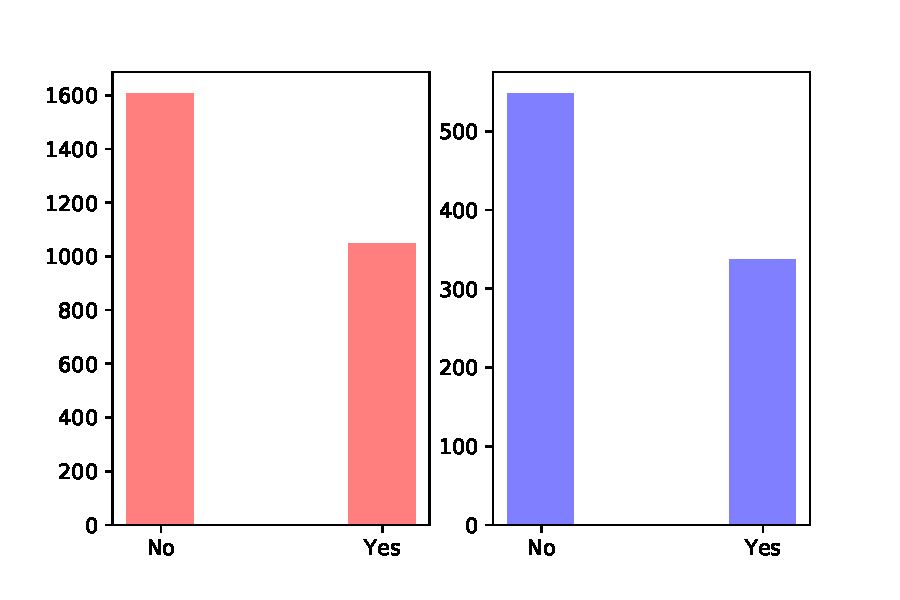
\includegraphics[width=1.1\columnwidth]{Figures/distribution.pdf}
    \caption{Distribution of relevance on train and test set}
    \label{fig:fig1}
\end{figure}

\subsubsection{Naive Bayes}
The simplest model that we tried was \textit{Naive Bayes} which assumes that words in the sentence are independent.
The results we obtained are shown in Table~\ref{tab:tab1}.

\begin{table}[h]
    \centering
    \begin{tabular}{ c | c c c c } 
         & Accuracy & Precision & Recall & F1 \\ 
         \hline
         Relevance & 0.84 & 0.79 & 0.79 & 0.79 \\
         Categories & 0.70 & / & / & 0.68 \\
    \end{tabular}
    \caption{Evaluation of Naive Bayes}
    \label{tab:tab1}
\end{table}

Although the model is naive, the results we got are not that bad.
The AUC of the model for predicting the relevance of the text is 91\%.

\subsubsection{Logistic Regression}
The results of Logistic Regression model are in Table~\ref{tab:tab2}.

\begin{table}[h]
    \centering
    \begin{tabular}{ c | c c c c } 
         & Accuracy & Precision & Recall & F1 \\ 
         \hline
         Relevance & 0.85 & 0.84 & 0.75 & 0.79 \\
         Categories & 0.73 & / & / & 0.72 \\
    \end{tabular}
    \caption{Evaluation of Logistic Regression}
    \label{tab:tab2}
\end{table}

The performance is similar to \textit{Naive Bayes}.
But we go the AUC of 92\% which is the highest of all baseline models.

\subsubsection{Support Vector Machine}
The results we got with this model are in Table~\ref{tab:tab3}.

\begin{table}[h]
    \centering
    \begin{tabular}{ c | c c c c } 
         & Accuracy & Precision & Recall & F1 \\ 
         \hline
        Relevance & 0.86 & 0.84 & 0.79 & 0.81 \\ 
        Categories & 0.74 & / & / & 0.73 \\
    \end{tabular}
    \caption{Evaluation of Support Vector Machine}
    \label{tab:tab3}
\end{table}

Overall SVM performed the best so we will use it in further experiments.
We also plotted the ROC curve for predicting the relevance of the text which is shown on Figure~\ref{fig:fig2}.

\begin{figure}[h]
    \centering
    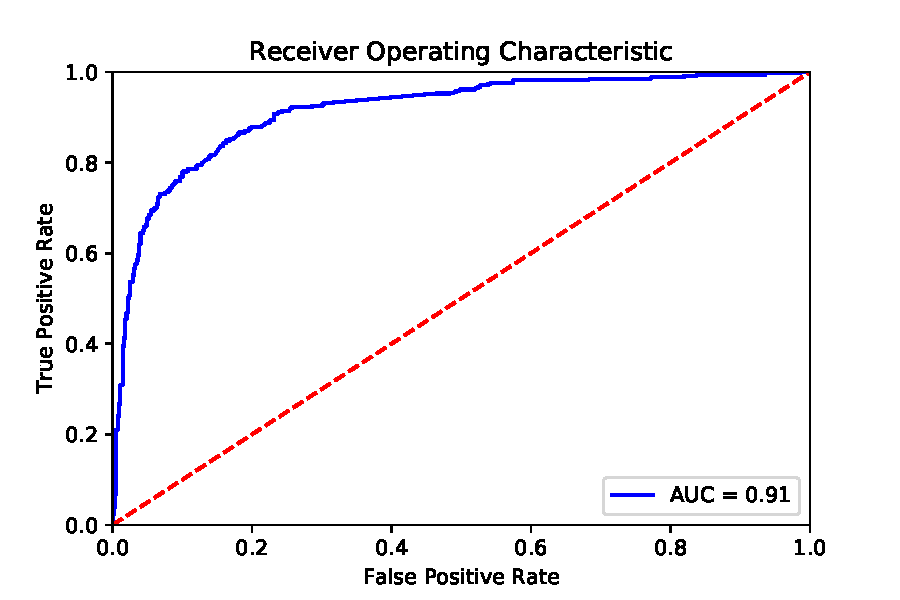
\includegraphics[width=1.0\columnwidth]{Figures/rocsvm.pdf}
    \caption{ROC curve of SVM performance}
    \label{fig:fig2}
\end{figure}

\subsection{Detecting of conversation drift}
To detect when the teacher needs to intervene we trained two models.
They were trained using the lemmatized texts as before.
But in this case we took sequential texts to train and test our models.
For training we took first 70\% of lemmatized texts and calculate their Tf-idf vectors.
From the experiments above we decided to train SVM model for classification of relevance of the text and Linear Regression (LR) for classification of category.
Both of the models were trained and evaluated using the 5-fold cross validation.
The accuracy and F1 score of SVM model were 0.83 and 0.82 respectively.
For the LR model we obtained 0.65 accuracy and 0.67 F1 score.

The last 30\% of conversations we used as to detect the drift.
We took the baches of 10 sequential messages and for each we predicted the relevance label.
We counted the number of relevance chats in a bach using the following method.
If the label was positive ('Yes') we counted it as relevant.
If the label was negative ('No') we also predicted the category.
We defined three soft categories ('C','S','M') which also count as relevant.
If the category was any of those we classified chat as relevant otherwise as non-relevant.
From the frequency of relevant/non-relevant chats we classified each bach.
The drift is detected if there is non relevant discussion in 5 consecutive baches.

\section{Future work}

For the future work we will focus on implementing some of the more advanced approaches to text classsification like using recurrent neural networks or transformers.
We will test some already trained embeddings and possibly train our own.
We will focus more in depth into the areas of identifying book relevance and message category type.



% \bibliographystyle{IEEEtran}
\bibliographystyle{acl_natbib}
\bibliography{bibliography}

\end{document}


